\documentclass{standalone}
\usepackage{tikz}
\usetikzlibrary{calc}
\begin{document}
    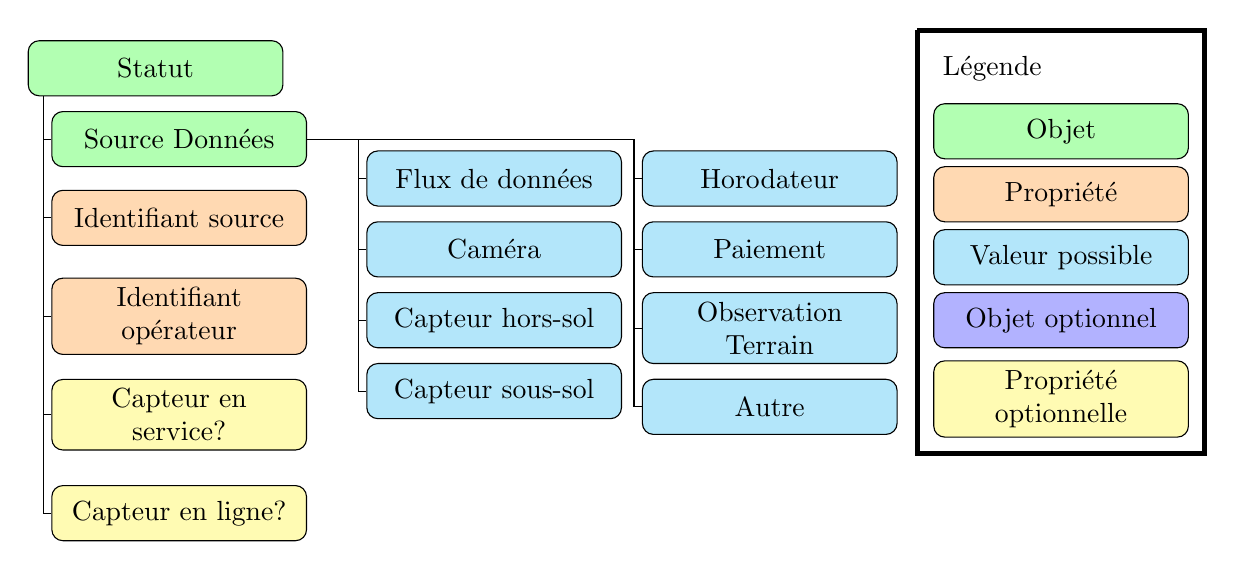
\begin{tikzpicture}
        \tikzstyle {objet} = [rectangle, rounded corners, text width=3cm, minimum height=0.7cm,text centered,  draw=black, fill=green!30]
        \tikzstyle {objet_opt} = [rectangle, rounded corners, text width=3cm, minimum height=0.7cm,text centered,  draw=black, fill=blue!30]
        \tikzstyle {propriete} = [rectangle, rounded corners, text width=3cm, minimum height=0.7cm,text centered,  draw=black, fill=orange!30]
        \tikzstyle{propriete_opt} =[rectangle, rounded corners, text width=3cm, minimum height=0.7cm,text centered,  draw=black, fill=yellow!30]
        \tikzstyle{enumeration} = [rectangle, rounded corners, text width=3cm, minimum height=0.7cm,text centered,  draw=black, fill=cyan!30]
        \node (statut) [objet] {Statut};
        
        \node (source_donnee) [objet, below of=statut,xshift=0.3cm,yshift=0.1cm]{Source Données};
        \node (flux_donnees) [enumeration, right of=source_donnee,xshift=3cm,yshift=-0.5cm]{Flux de données};
        \node (camera) [enumeration,below of=flux_donnees,yshift=0.1cm]{Caméra};
        \node (above_ground) [enumeration, below of=camera,yshift=0.1cm]{Capteur hors-sol};
        \node (in_ground) [enumeration, below of=above_ground,yshift=0.1cm]{Capteur sous-sol};
        \node (meter) [enumeration, right of=flux_donnees,xshift=2.5cm]{Horodateur};
        \node (paiement) [enumeration, below of=meter,yshift=0.1cm]{Paiement};
        \node (in_person) [enumeration, below of=paiement]{Observation Terrain};
        \node (autre_obs) [enumeration, below of=in_person]{Autre};
        \draw (flux_donnees.west) -| ++(-.1,.1) |- (source_donnee);
        \draw (flux_donnees.west) -| ++(-.1,-.1) |- (camera);
        \draw (camera.west) -| ++(-.1,-.1) |- (above_ground);
        \draw (above_ground.west) -| ++(-.1,-.1) |- (in_ground);
        \draw (meter.west) -| ++(-.1,.1) |- (source_donnee);
        \draw (meter.west) -| ++(-.1,.1) |- (paiement);
        \draw (in_person.west) -| ++(-.1,.1)|-(paiement);
        \draw (in_person.west)-| ++(-.1,.1)|- (autre_obs);

        \node (id_source) [propriete,below of=source_donnee] {Identifiant source};
        \node (id_operateur) [propriete, below of=id_source,yshift=-0.25cm] {Identifiant opérateur};
        \node (capteur_service) [propriete_opt,below of=id_operateur,yshift=-0.25cm]{Capteur en service?};
        \node (capteur_enligne) [propriete_opt, below of=capteur_service,yshift=-0.25cm]{Capteur en ligne?};
        \draw (capteur_enligne.west) -| ++(-0.1,0.1) |- (capteur_service);
        \draw (capteur_service.west) -| ++(-0.1,0.1) |- (id_operateur);
        \draw (id_operateur.west) -| ++(-0.1,0.1) |- (id_source); 
        \draw (id_source.west) -| ++(-0.1,0.1) |- (source_donnee);
        \draw (source_donnee.west) -| ++(-0.1,0.1) |- ($(source_donnee.west |- statut.south) + (-0.1,0)$);
        \node (legend) [text width =3cm,right of=statut, xshift=10.5cm]{Légende};
        \node (obj_leg) [objet, below of=legend,yshift=0.2cm]{Objet};
        \node (prop_leg) [propriete, below of=obj_leg,yshift=0.2cm]{Propriété};
        \node (enum_leg) [enumeration , below of=prop_leg,yshift=0.2cm]{Valeur possible};
        \node (obj_opt_leg) [objet_opt, below of=enum_leg,yshift=0.2cm]{Objet optionnel};
        \node (propriete_opt_leg) [propriete_opt, below of=obj_opt_leg]{Propriété optionnelle};
        \coordinate (legend_box_top_left) at ($(legend.north west) + (-0.2,0.2)$);
        \coordinate (legend_box_bottom_right) at ($(propriete_opt_leg.south east) + (0.2,-0.2)$);
        \draw[line width=2pt] (legend_box_top_left) -| (legend_box_bottom_right) -| (legend_box_top_left);
    \end{tikzpicture}
\end{document}